\documentclass[titlepage, a4paper, 11pt, dvipdfmx]{jsarticle}
\usepackage{customstyle}

\title{\Huge【レポート\#3 IAM】}
\date{\today}%日付
\author{\Large BV20036 \quad 大野 弘貴}%名前

\begin{document}
\maketitle
\pagenumbering{roman}
% \tableofcontents%目次が消したい場合はコメントアウト
\newpage
\pagenumbering{arabic}

%%%%%%%%%%%%%%%%%%%%%%%%%%%%%%%%%%%%%%%%%%%%%%%%%%%%%%%%%%%%%%%%%%%%%%%%%%%%%
%%%%%%%%%%%%%%%%%%%%%%%%%%%%%%%%%%%%%%%%%%%%%%%%%%%%%%%%%%%%%%%%%%%%%%%%%%%%%
%%%%%%%%%%%%%%%%%%%%%%%%%%%%%%%%%%%%%%%%%%%%%%%%%%%%%%%%%%%%%%%%%%%%%%%%%%%%%
%以下サンプル%ここから書き始めてください

%セクション(目次に表示されるのは初期設定では)

Theorem
\begin{align} 
  \left\{f(x)g(x)\right\}' 
  &= \lim_{h\rightarrow 0}\frac{f\left(x+h\right)g\left(x+h\right)-f\left(x\right)g\left(x\right)}{h}\\\ 
\end{align}
Proof. \\
From defnition
\begin{align}  
  & \ \ \ \ \ \ f\left(x+h\right)g\left(x+h\right)-f\left(x\right)g\left(x\right)\\\
   &= f\left(x+h\right)g\left(x+h\right){-f(x)g(x+h)+f(x)g(x+h)}-f\left(x\right)g\left(x\right)\\\ 
   &= \left(f\left(x+h\right)-f(x)\right)g\left(x+h\right)+\left(g(x+h)-g\left(x\right)\right)f\left(x\right)\\\ 
\end{align}
Thus
\begin{align} 
  & \ \ \ \ \ \ \frac{f\left(x+h\right)g\left(x+h\right)-f\left(x\right)g\left(x\right)}{h} \\\ 
  &= \frac{\left(f\left(x+h\right)-f(x)\right)g\left(x+h\right)+\left(g(x+h)-g\left(x\right)\right)f\left(x\right)}{h}\\\ 
  &= \frac{f\left(x+h\right)-f(x)}{h}g\left(x+h\right)+\frac{g(x+h)-g\left(x\right)}{h}f\left(x\right)\\\ 
\end{align}
Therefore
\begin{align}  
  & \ \ \ \ \ \ \lim_{h\to 0}\frac{f\left(x+h\right)g\left(x+h\right)-f\left(x\right)g\left(x\right)}{h} \\\ 
  &= \lim_{h\to0}\frac{f\left(x+h\right)-f(x)}{h}g\left(x+h\right)+\lim_{h\to0}\frac{g(x+h)-g\left(x\right)}{h}f\left(x\right)\\\ 
\end{align}



\begin{align} \left\{\frac{1}{g(x)}\right\}' 
  &= \lim_{h\rightarrow 0}\frac{\frac{1}{g\left(x+h\right)}-\frac{1}{g\left(x\right)}}{h}\\\ 
  &= \lim_{h\rightarrow 0}\frac{1}{h}\left(\frac{1}{g\left(x+h\right)}-\frac{1}{g\left(x\right)}\right)\\\ 
  &= \lim_{h\rightarrow 0}\frac{1}{h}\frac{g(x)-g(x+h)}{g\left(x+h\right)\cdot g(x)}\\\ 
  &= \lim_{h\rightarrow 0}\frac{g(x)-g(x+h)}{h}\cdot\frac{1}{g\left(x+h\right)\cdot g(x)}\\\ 
  &= \lim_{h\rightarrow 0}\left(-\frac{g(x+h)-g(x)}{h}\right)\cdot \lim_{h\rightarrow 0}\left(\frac{1}{g\left(x+h\right)\cdot g(x)}\right)\\\ 
  &= -g'(x)\cdot \left(\frac{1}{g\left(x\right)\cdot g(x)}\right)\\\ &= -g'(x)\cdot \left(\frac{1}{g^2(x)}\right)\\\ \end{align}


\begin{itembox}[l]{囲いのタイトル左版}

    \scalebox{0.65}{
        \begin{tabular}{|c|c|c|c|c|c|c|c|c|c|c|c|c|c|c|c|c|c|c|c|c|}
        \hline
        x & 1 & 2 & 3 & 4 & 5 & 6 & 7 & 8 & 9 & 10 & 11 & 12 & 13 & 14 & 15 & 16 & 17 & 18 & 19 & 20\\ \hline
        y & 0.98 & 7.61 & 2.47 & 1.38 & 3.31 & 0.83 & 6.72 & 8.07 & 9.83 & 6.36 & 14.3 & 21.0 & 20/9 & 14.7 & 12.3 & 20.0 & 13.0 & 20.7 & 17.7 & 23.8\\ \hline
        \end{tabular}
    }

 

    \begin{itemize}
        \item コレスキー分解およびQR分解を用いた最小二乗法で上のデータを近似する多項式(の係数) を求め,与えられたデータと得られた多項式を重ねたグラフを作成せよ。 多項式の次数はn=1, 7, 9, 11, 13の5つの場合についてそれぞれ行うこと。
        \item n=1, 7, 9, 11, 13のそれぞれの場合について,コレスキー分解およびQR分解を用いて得られた 解 および, に対し,
        \begin{itemize}
            \item 正規方程式の相対残差2ノルム: $ \| r_{chol/qr} \|_2 = \| A^T b - A^T Ax_{chol/qr} \|_2 / \|\| b \|\| $ 
            \item 元の最小二乗問題の相対残差2ノルム:$ \| r_{chol/qr} \|_2 = \| b - x_{chol/qr} \|_2 / \| b \|_2 $ 
        \end{itemize} 
        \item 【任意】上記に加えて,特異値分解を用いた解法についても上記を行い比較せよ。
  \end{itemize}
\end{itembox}
    \section{コレスキー分解とは}
    A が正定値対称行列のとき, A は下三角行列 L = ($l_ij$ ) を用いて

    $$ A=LL^T $$

    の形に分解できる。この分解をコレスキー分解という。

A =  $LL^T$ = \(
        \left(
        \begin{array}{ccc}
        l_{11} & 0 & 0 \\
        l_{21} & l_{22} & 0 \\
        l_{31} & l_{32} & l_{23}
        \end{array}
        \right)
        \)
       \(
            \left(
            \begin{array}{ccc}
            l_{11} & l_{21} & l_{31} \\
            0 & l_{22} & l_{32} \\
            0 & 0 & l_{23}
            \end{array}
            \right)
    \)

        ただし、$l_{ii}>0$とする。

\section{QR分解とは}
QR分解は行列分解の1つで以下の定理のことである。

\begin{itembox}[l]{囲いのタイトル左版}
    \begin{equation}
        A \in \mathbb{N}
    \end{equation}
    と一意に分解できる。ただし、Q $\in$ $\mathbb{R}^{n \times n} $ は対角成分が正となる上三角行列である。
\end{itembox}


\section{実行結果}

\begin{figure}[H]
    \begin{center}%中央寄せ用
      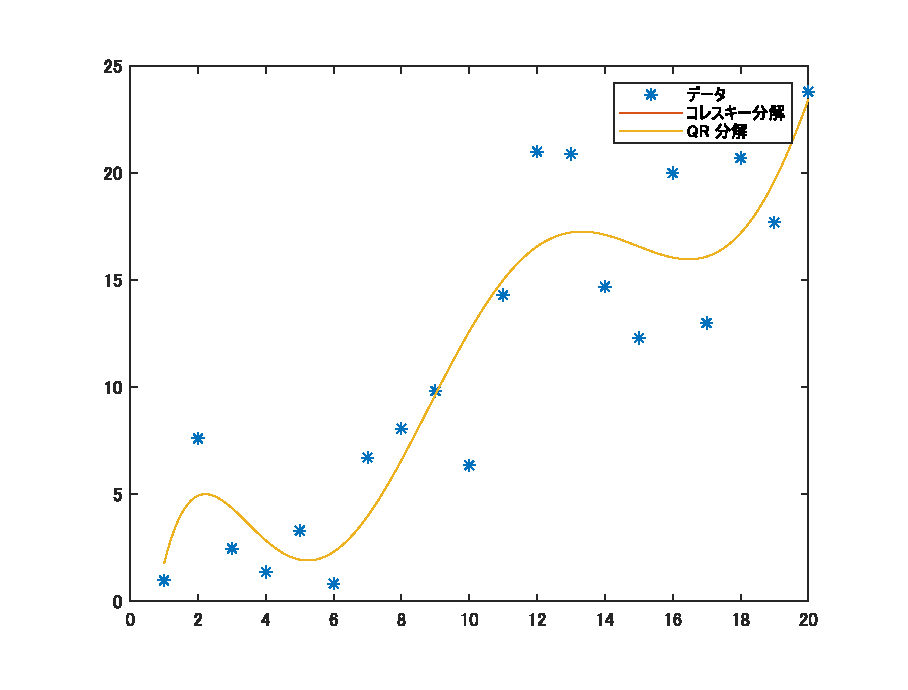
\includegraphics[width=13.5cm]{./graphics/saisyounijouhou/7.eps}
    \caption{キャプション}
    \label{Label}%ラベル
    \end{center}
  \end{figure}

  \begin{figure}[H]
    \begin{center}%中央寄せ用
      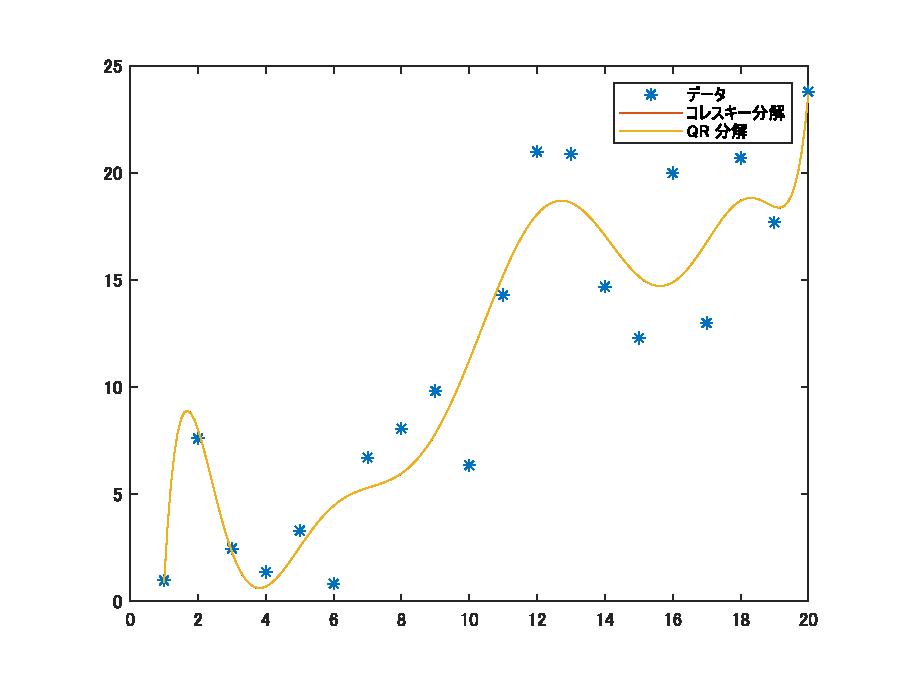
\includegraphics[width=13.5cm]{./graphics/saisyounijouhou/9.eps}
    \caption{キャプション}
    \label{Label}%ラベル
    \end{center}
  \end{figure}


  \begin{figure}[H]
    \begin{center}%中央寄せ用
      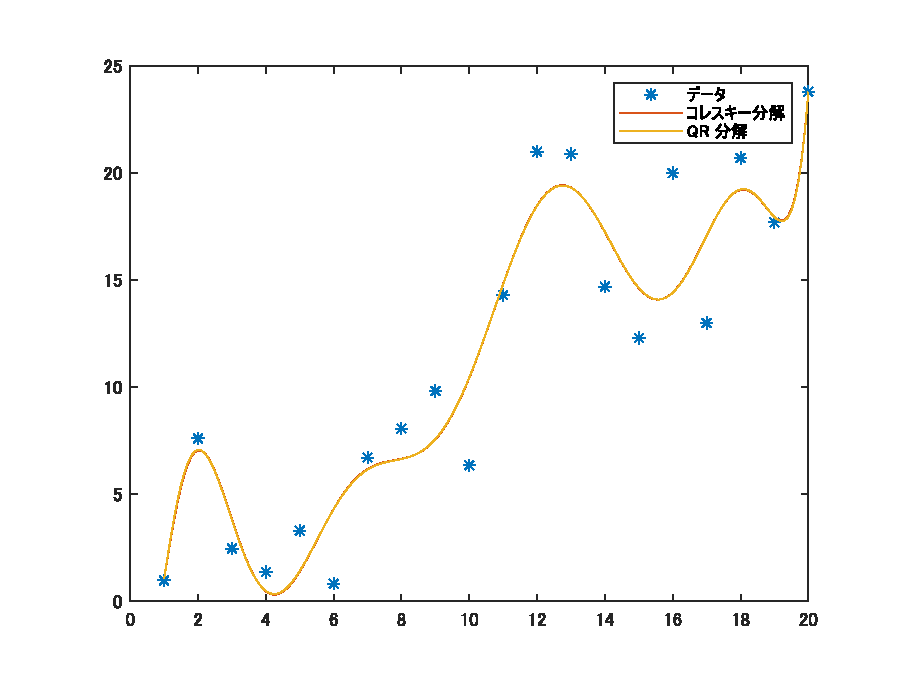
\includegraphics[width=13.5cm]{./graphics/saisyounijouhou/11.eps}
    \caption{キャプション}
    \label{Label}%ラベル
    \end{center}
  \end{figure}


  \begin{figure}[H]
    \begin{center}%中央寄せ用
      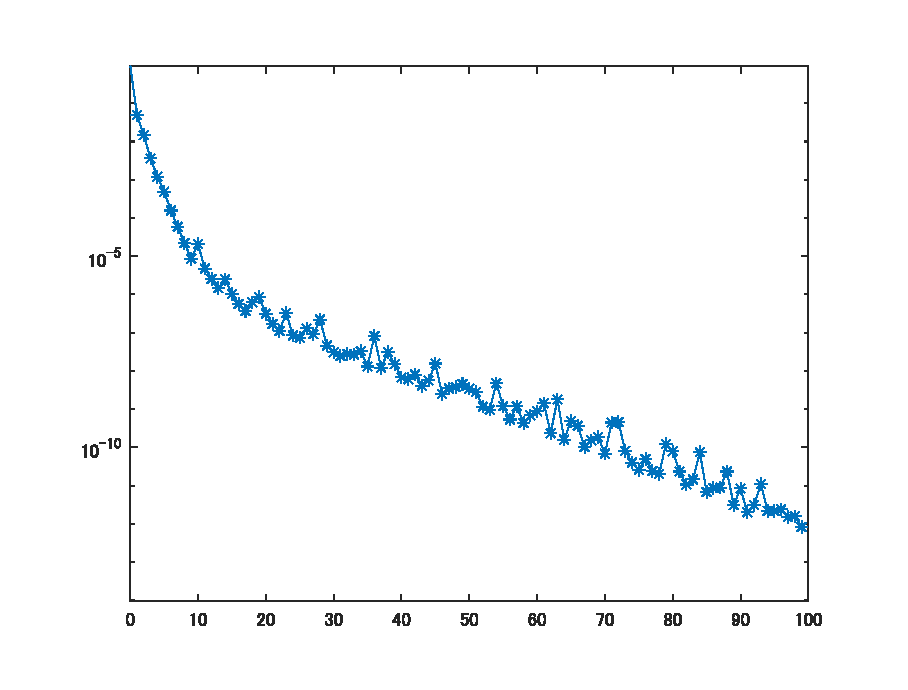
\includegraphics[width=13.5cm]{./graphics/100.eps}
    \caption{キャプション}
    \label{Label}%ラベル
    \end{center}
  \end{figure}

\section{考察}
 実行結果を見ると、コレスキー分解・QR分解ともにnの値を大きくするにつれて残差の値が小さくなっているので、nの値を増やせばより真の値に近づくことが分かる。またQR分解より最小二乗法のほうがnの値を大きくしたときより小さくなったので、最小二乗法のほうが精度がよかった。もしくは標本点との相性がよかったかもしれない。

\section{破綻する原因}
 今回用いた数値解法は前提として、求める行列が正定値対称行列である必要があるが、nの値を大きくするとこのせい値対称行列を満たさない場合が現れた。これによってコレスキー分解ができず最小二乗法を行うことができなかった。
\end{document}
